%results 05-20 18-50.mat
\subsection{Badania przesiewowe dla dużej ilości neuronów}
Eksperyment miał na celu sprawdzenie jak zachowuje się sieć przy dużej ilości neuronów w dwóch warstwach. Wszystkie parametry pozostały bez zmian, zmieniana była jedynie ilość neuronów w zakresie od 100 do 400 z krokiem 50.
\begin{figure}[!h]
\centering
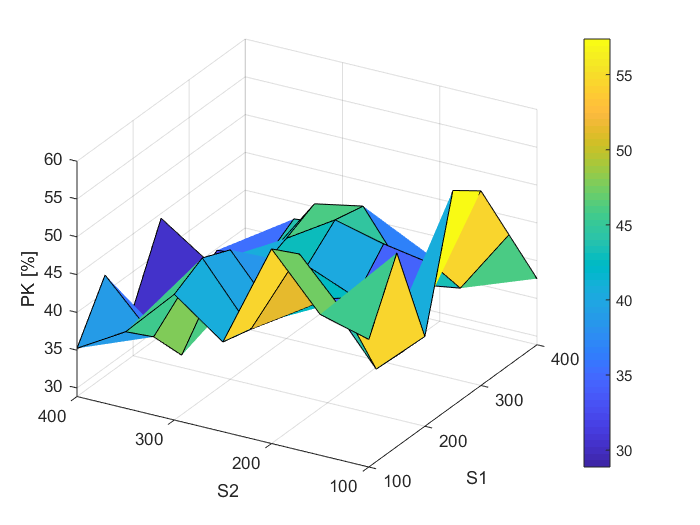
\includegraphics[width = 0.7\textwidth]{Grafika/PK_duze.png}
\caption{Wpływ liczby neuronów w warstwie pierwszej i drugiej na poprawność klasyfikacji}
\label{fig:PKeksperyment2}
\end{figure}
\begin{figure}[!h]
\centering
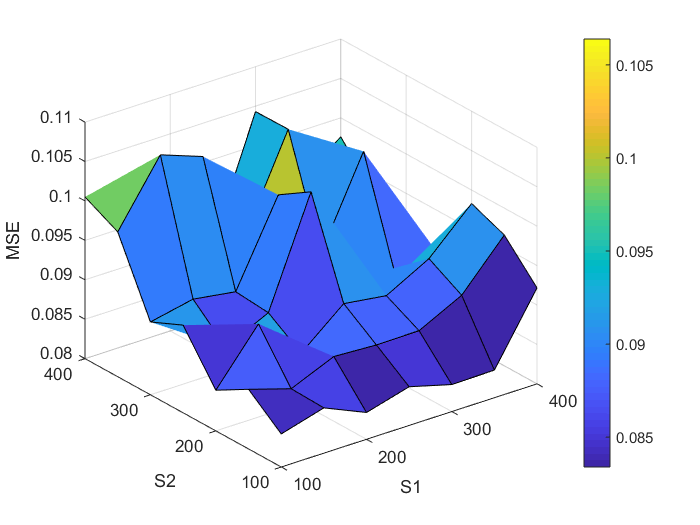
\includegraphics[width = 0.7\textwidth]{Grafika/MSE_duze.png}
\caption{Wpływ liczby neuronów w warstwie pierwszej i drugiej na błąd średnio-kwadratowy}
\label{fig:MSEeksperyment2}
\end{figure}
\clearpage
Największą poprawność klasyfikacji ($57.38\%$) uzyskano dla 250 neuronów w warstwie pierwszej i 100 w warstwie drugiej.\\
Najmniejszy błąd średnio-kwadratowy ($0.0834284$) osiągnięty został dla 300 neuronów w warstwie pierwszej i 100 neuronów w warstwie drugiej. Dla tej konfiguracji $PK$ wyniosło $54.63\%$.\\
Na podstawie powyższych obserwacji można wyciągnąć wniosek, iż duża liczba neuronów niekoniecznie wpływa pozytywnie na proces uczenia sieci. Poprawność klasyfikacji zawierała się w większości w przedziale $45-55\%$.
